\documentclass[11pt]{article}

\usepackage{graphicx, amsmath, amsfonts, amssymb, microtype, fullpage, url, algorithm, algorithmic, hyperref, longtable}
\newcommand{\argmax}{\operatornamewithlimits{argmax}}
\setlength{\parskip}{5pt}

\title{Project Report - Classification of questions on stackoverflow\\ Machine Learning, Fall 2012}
\author{Luke Vilnis, Annamalai Natarajan, Ariel Kobren}

\begin{document}
\sloppy

\maketitle

\section{Problem Statement}

``What is the best programming language?'' There are too many
answers to this question and very little consensus among programmers
as well. The problem being the question is too broad and the answers
will almost never satisfy all subgroups. But, how do we train a
classifier to predict if a question is too broad? In general, how can a
classifier detect if a question is relevant given some target
audience. In this project we are interested in predicting if a
question asked on Stackoverflow (target audience) will be closed (not
relevant to this community of users).

\noindent Stackoverflow \cite{website:stackoverflow} is a forum where
users ask software and programming related questions which are
subsequently answered by other users in the forum. Now, there are
instances when questions posed by users do not meet the requirements
set by the moderators and hence are `closed'. Stackoverflow predicts
that anually 6\% of its questions are closed. If only the users knew
well ahead of time that the chances of their question being closed is
high, then, the user could rephrase or research the question before
actually posting the question on the forum.

\begin{figure}
\centering
\fbox{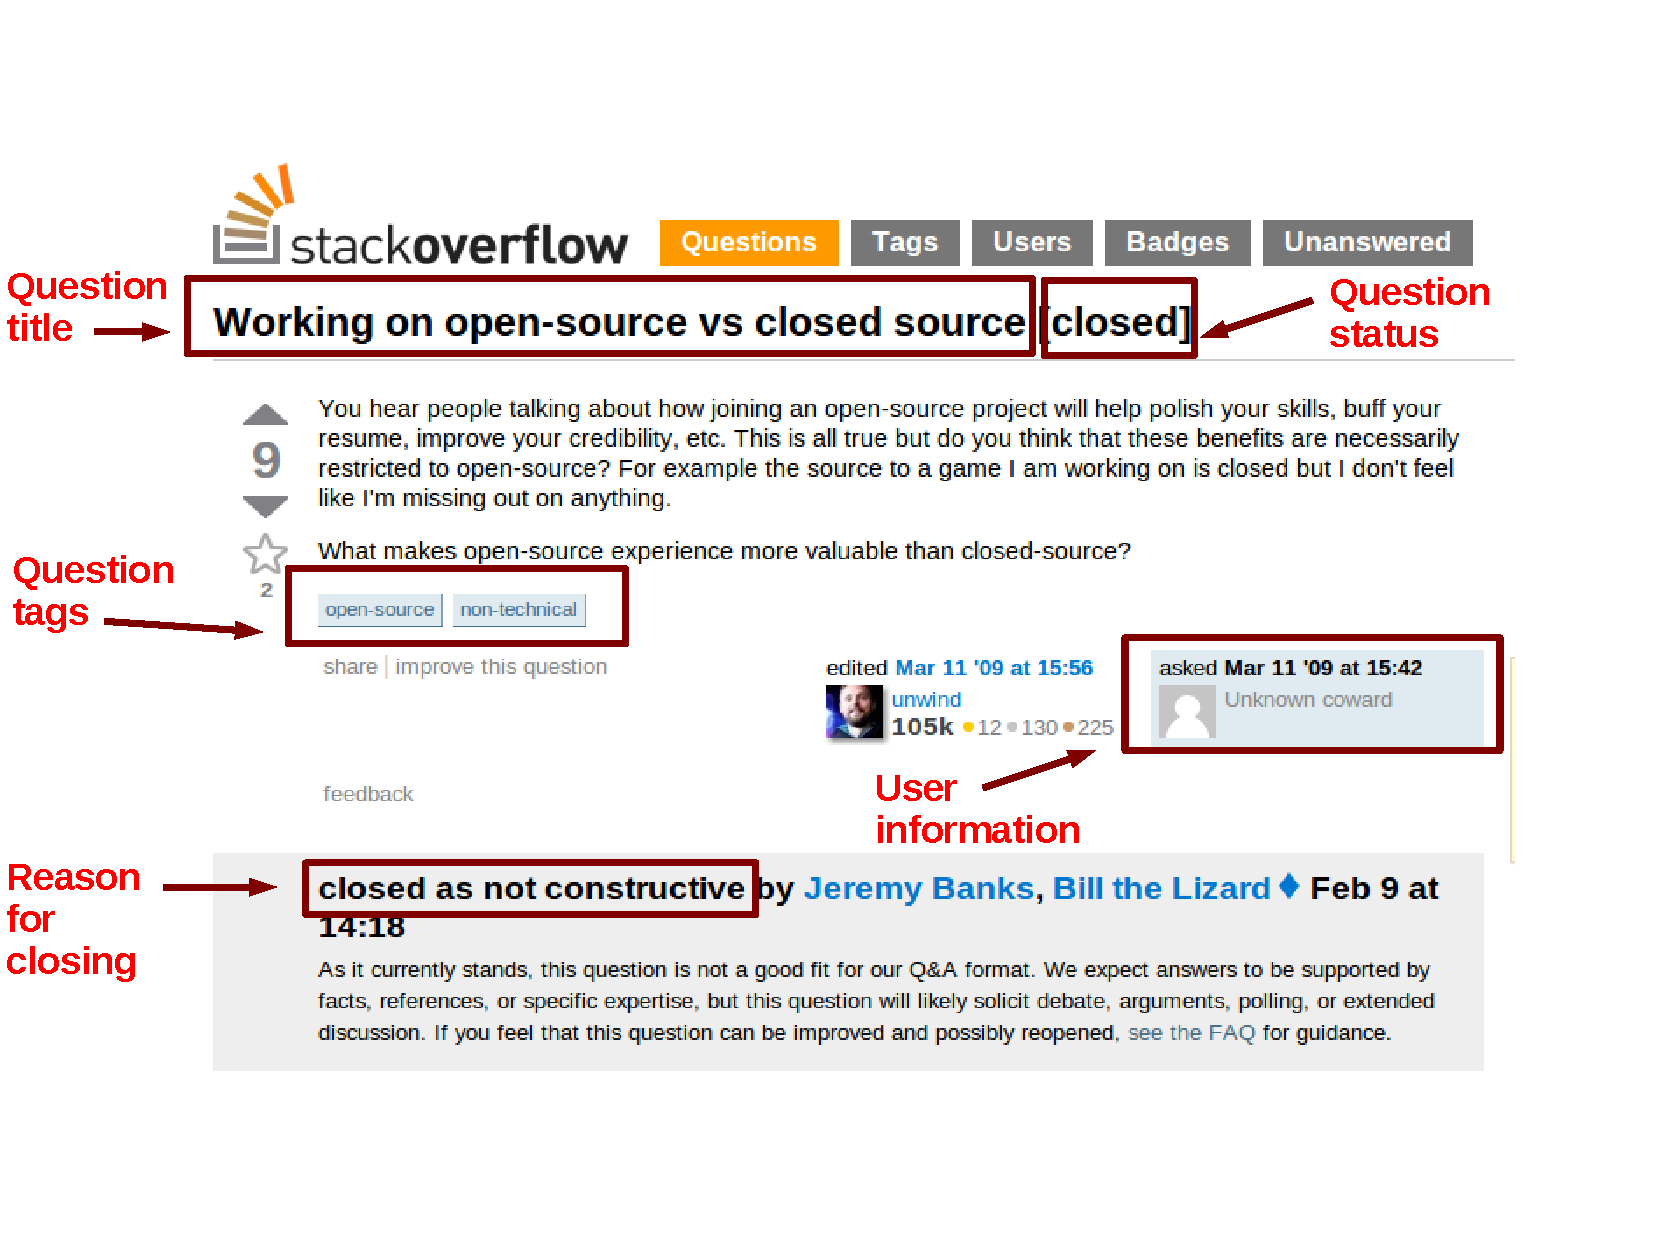
\includegraphics[width=4in,height=3.5in]{images/example_label.pdf}}
\caption{Sample closed question}
\label{fig:sample}
\end{figure}

\noindent According to Stackoverflow's policies, a question maybe
closed if it falls into one of the five categories listed below:

\begin{itemize}
\item \textbf{Exact duplicate}: This is exactly as it phrased. If a similar question has already been asked in the past then the question is not novel in any way
\item \textbf{Off-topic}: Like we mentioned above stackoverflow is a forum for software and programming related questions and so off-topic questions are most likely closed. e.g. From the Brain imaging toolbox, AFNI, I see lots of activity in the Dorso Lateral pre-frontal cortex, does it mean that part of the brain is involved in activity A?
\item \textbf{Not constructive}: Questions get closed under this category when they solicit opinion, debate, arguments, polling, or extended discussion. Our opening question on "What is your favorite programming language?" is a good example
\item \textbf{Note a real question}: When questions are ambiguous, vague, incomplete, overly broad or rhetorical. e.g. `Sort HTML attributes with JavaScript' - this user does not reveal problem encountered when attempting to perform this task
\item \textbf{Too localized}: If the question asked pertains to one specific problem which occurs in a specific setting and will not benefit future users of the forum. e.g. a question pertaining to an obsolete java query
\end{itemize}

\noindent Refer to figure \ref{fig:sample} for a sample of closed question. In our data analysis we have deliberately eliminated questions that fall under `Exact duplicate' category. The reason being that these are valid questions but they have already been asked before. Elimination of duplicate questions is  also less likely to confuse the classifier when attempting to tease apart closed from open questions based on structral information from questions.

\section{Data set}
In our initial work, we used a data set collected using
Stackoverflow's \emph{StackExchange Data Explorer}
\cite{website:stackexchange}. This online tool
allows users to query raw data directly from
Stackoverflow. Specifically, we issued the following commands:

\begin{verbatim}
SELECT * FROM posts WHERE PostTypeId=1 AND CreationDate > '20110813'
    AND ClosedDate > '20110813';

SELECT * FROM posts Where PostTypeId=1 AND CreatedDate > '20110813'
    AND ClosedDate IS NULL;
\end{verbatim}

These two queries aim to retrieve all questions (PostTypeId=1) posted
on Stackoverflow on or after August 13$^{\textrm{th}}$, 2011 that: 1)
were closed on or after August 13$^{\textrm{th}}$ and 2) have not been
closed, respectively.  However, as a matter of policy, the Data
Explorer will not return more than 50,000 rows at a time.  Thus, after
issuing these two queries, we had collected a data set of 50,000
questions that had been closed (55MB) and 50,000 that were still open as of
query issue date (75MB).

The data was formatted as CSV files and contained the following
fields: Question Id, PostTypeId, AcceptedAnswerId, ParentId,
CreationDate, Score, ViewCount, Body, OwnerUserId, LastEditorUserId,
LastEditorDisplayName, LastEditDate, LastActivityData, Title, Tags,
AnswerCount, CommentCount, FavoriteCount, ClosedDate and
CommunityOwnedDate. Of these fields, the fields that we worked with
were in our initial testing were:

\begin{enumerate}
  \item Body - the raw text of the question
  \item Tags - user provided question categories (e.g. Java,
    algorithms, etc.)
\end{enumerate}

To parse the CSV files collected, we used third party CSV Praser from
SuperCSV, written in Java \cite{website:supercsv}.

Midway through our experiments, we discovered a \emph{Kaggle}
competition for predicting closed questions on \emph{Stackoverflow}
\cite{website:kaggle}. The competition materials included larger data sets: a
sample train set (133MB) and a larger train set (3.5G).  These data
files were also formatted as CSV files however included different
question fields: PostId, PostCreationDate, OwnerUserId,
OwnerCreationDate, ReutationAtPostCreation,
OwnerUndeletedAnswerCountAtPostTime, Title, BodyMarkdown, Tag1, Tag2,
Tag3, Tag4, Tag5, PostClosedDate and OpenStatus.

\subsection{Pre-processing}
To get the data in workable form, a number of pre-processing steps
were required. First, the ``body'' field, which contained the text of
each question, was formatted as HTML and had to be
cleaned (i.e. HTML tags stripped). Additionally, images and code were
removed.  We had to remove code because it is highly variable
(variables always have different names) and it contains a number of
strange characters and formatting.

Additionally, there were a few components of a question whose presence
usually indicated that the question would be closed.  For example, the
body of a question can include a \begin{verbatim}
  <strong> \end{verbatim} tag which indicates that a Stackoverflow
moderator (who have the power to close posts) has commented on the
question. These tags showed a large positive correlation to closed
questions and thus, needed to be removed. Similarly, all ``Possible
duplicate'' or ``Closed'' notes, attached to a question, needed to be
removed.  Finally, any urls, which usually hyperlinked to a similar
question on Stackoverflow, were removed.

After being cleaned, the text of each question was tokenized.

\subsection{Features}

For each question, two categories of features were extracted and used
for training: features extracted from the body of the question and
features extracted concerning the metadata of that particular
question. As metadata features, the following fields were extracted:

\begin{itemize}
  \item Bucketed question length (in characters); a binary feature
    taking the value '1' if the questions has more than 1000 characters
  \item Question tags; converted to a list of strings and concatenated
    onto each feature vector
\end{itemize}

Before extracting features from question bodies, first, each question
body was down-cased and tokenized (using Stanford's NLP Java library)
\cite{stanfordnlp}. Then, the count of each unigram, bigram and
trigram, per question, was added to each feature vector. Finally, the
cross product of all tags and distinct unigrams, per question, was
added to each feature vector.  Using both the metadata and ngram
features, each feature vector was on the order of 2.5 million features
long.

\section{Methods}
\begin{itemize}
\item using factorie facilities for storing instances, trimming domains, learning classifiers, judging accuracy, info gain, etc. Need sparse vectors cause lots of data. pretty fast sgd implementations
\item Use information gain to see suspicious features
\end{itemize}

\section{Results}
\begin{itemize}
\item 71\% accuracy with logistic regression trained using AdaGrad (not l2 regularized but effectively regularized since its an online learning algorithm). SVM, naive bayes, l2 log reg etc does slightly worse.
\item Naive bayes was winner until we added cross product
  features. High bias/low variance does better
  \item How long did it take run the whole thing?
\end{itemize}

\begin{figure}
\centering
\fbox{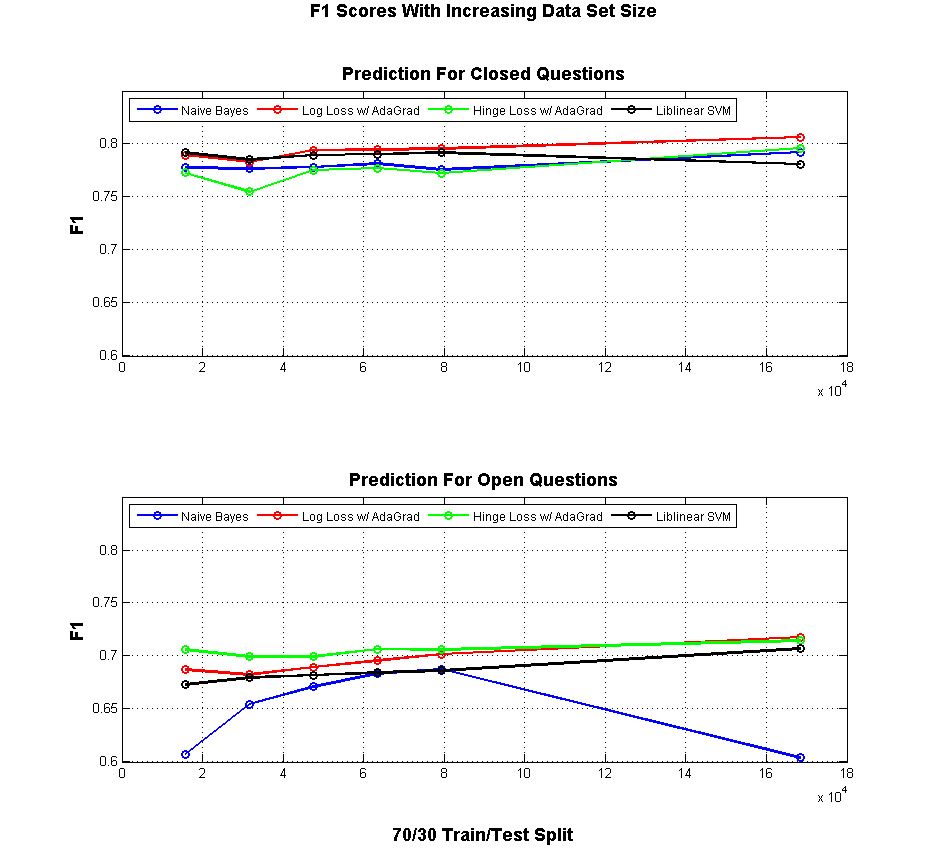
\includegraphics[width=6.5in,height=6in]{images/stackoverflow_results}}
\caption{Classifier accuracies in predicting closed questions}
\label{fig:results}
\end{figure}

\section{Discussion}

\begin{itemize}
  \item Ngrams didn’t help - need smarter features - we get 100\%
    almost train set accuracy, so the problem is bad features, not
    inability to fit. Regularization also doesn’t help much at all
    (tried manually grid searching l2 lambda). Overfitting is not the
    problem.
  \item using information gain to figure out which features were best
  \item What where the best features? Why were they best?
  \item What was the best classifier, why?
\end{itemize}

\section{Future directions}
\begin{itemize}
\item Use kaggle data set (which we have); 70 million training instances, 80 thousand test instances
\item We’ll need to split up the data (because it’s big) to be able to use it; we’re planning to learn the weights of our linear classifier using stochastic gradient descent (blocked-adagrad)
\item Add more features (TFIDF, other NLP features), heuristic of adding number of rare words from Alex’s paper
\item Try out new classifiers - random forests
\item Try things besides open/closed - like answered/unanswered
\end{itemize}

\bibliography{bib}{}
\bibliographystyle{plain}

\end{document}
